\documentclass[hidelinks, a4paper]{report}
\usepackage[english]{babel}
\usepackage[utf8]{inputenc}
\usepackage[T1]{fontenc}
\usepackage{verbatim}
%%Comments
%Use \myquote{word} for correct quotation marks on word.

%%Packages
\usepackage{hyperref}
\usepackage{graphicx}
\usepackage{pdfpages}
\usepackage{supertabular}
\usepackage{float}
\usepackage{todonotes}
\usepackage{wrapfig}
\usepackage{lineno}
%\usepackage[moderate,margins=tight,marginwidth=3cm]{savetrees}

 
%%Commands
%Pretty tables
\renewcommand{\arraystretch}{1.5}
%Easy correct quotation
\newcommand{\myquote}[1]{``\emph{#1}''}
%command for complete references
\newcommand{\completeref}[1]{\ref{#1},~\nameref{#1}}
%commands for referencing lines to be used with lineno package
%Usage: enter \quotelabel{label} on the line with the quote
%Usage: type [Aa]ppendix \quoteref{label} when referencing the quote
%\newcommand{\quotelabel}[2]{\label{#1}\linelabel{#2}}
\newcommand{\quoteref}[2]{\completeref{#1}, line~\lineref{#2}}
%prettier chapters
\usepackage{titlesec, blindtext, color}
\definecolor{gray75}{gray}{0.75}
\newcommand{\hsp}{\hspace{20pt}}
\titlespacing*{\chapter}{0pt}{0pt}{20pt}
\titleformat{\chapter}[hang]{\Huge\bfseries}{\thechapter\hsp\textcolor{gray75}{|}\hsp}{0pt}{\Huge\bfseries}


%%Document start
\begin{document}

\title{An Examination of the Recruitment Process at Valcon}
\author{Jakob Ambeck Vase \and Jonas Kastberg Hinrichsen \and Jakob Merrild \and Michael Frikke Madsen \and Martin Juul Petersen}
\listoftodos[Todos]

%%Preface
\maketitle
\tableofcontents
%\listoffigures
%%Content
\chapter{Introduction}
\section{Problem introduction}

Processen skal identificeres, automatiseres og effektiviseres.
\todo{Be sure to mention Danni's goal (document the problem)}

\section{List of activities}
Based on the process analysis in which we identified the work areas relevant to the process, we conducted various interviews.
We chose to begin with interviewing Lisbeth (of accounting) and Peter (of IT), as they are the ones most affected by the process.
We chose to interview Hanne (NBA) as well, as she is the initiator of the process at Valcon.
Finally, we chose to observe both IT and accounting, to get a sense of the work flow there.

When we analyzed the data, we realized that we had to interview Jytte (process initiator at OMT) as well, as much of the problem originates in OMT.

Based on Valcons key values we were asked not to conduct a quantitative questionaire analysis of how the consultants experience the process (source appendix \ref{app:danni_initiation}). The process should however be transparent to them, and thus we deemed that the analysis would not have a greater impact on the overall data gathered.

\todo{Why no Valcon/OMT recruiter interview? SOURCE}

\section{Solutions Already Underway}
Valcon was aware that there was an issue in recruitment even before the project began.
A couple of years ago, the company changed its mail- and calendar platform from Lotus Notes to a Microsoft Exchange based solution. This meant that the old HR-system, a database in Notes, quickly became deprecated, as the information was only used during the hiring process, and not kept updated as before. This also meant that a lot of functionality that the fully integrated Notes system had, was lost.
There is a general knowledge that the situation is unstable, and that a lot of information is copy-pasted by hand, and a lot of data is not kept up to date in the way Valcon wants it to be.

Valcon is currently investigating possible new HR-systems to remedy this.

We have, during the course of this project, been aware that a solution to part of the problem was already underway, and we have had it in mind as we proposed our own solutions.

\section{Notes}
During the analysis we realized that OMT was an integral part of the problem, and started to analyze them as well. Our scope got too big, so we limited the amount of gathered knowledge from OMT to a single interview with a recruiter at OMT with a key person in regards to the process. 

We realize that this limits our general understanding of the procress, and thus most of the solutions proposed in regards to OMT are conducted based on limited knowledge, and should be further revised before implemented. 

\chapter{In-line analysis \\ Understanding Valcon}
The following chapter will present our understanding of Valcon and their business and how this relates to the problem. \todo{Not very good...}

\section{Environment}
\todo{Move to appendix and write summary} \todo{Sources!}
\subsection{Valcon's environment}
Valcon operates within an competitive environment where image is key. 
There's a major need for experienced and knowledgeable consultants but there's also a lot of competition in the field.
Due to this, Valcon's business strategy has been to hire the best and brightest employees and accept the fact that they're unable to be the cheapest organisation to hire,
but they pride themselves with being a company who follows their customers all the way to the finish line with the projects that they've been hired to do. 
They work hard trying to hire consultants within a wide range of fields, meaning there's a high chance that they have just the consultant a new project needs, no matter what field the project operates within. 
This means that Valcon is a company competing on quality and knowledge rather than on the price, meaning that Valcon is able to compete with other companies that might be fighting each other on the price.
\subsection{OMT's environment}
OMT operates within an environment where they aren't facing a lot of competition. 
There aren't many ship designers building war ships and this places OMT in a position where they need employees with that specific experience and there aren't many candidates, as most of these employees are most likely already employed somewhere else.
Because of this, OMT finds a lot of their workforce within other ship design companies. 
Since these other companies work in other fields where OMT doesn't, they don't mind subcontracting the employees that OMT wants, as this just gives them more work. 
\section{Valcon's business canvas}
The business canvas gives an overview of Valcon's business.
Based on our analysis we have the following understanding of Valcon's canvas.
\begin{figure}[!htp]
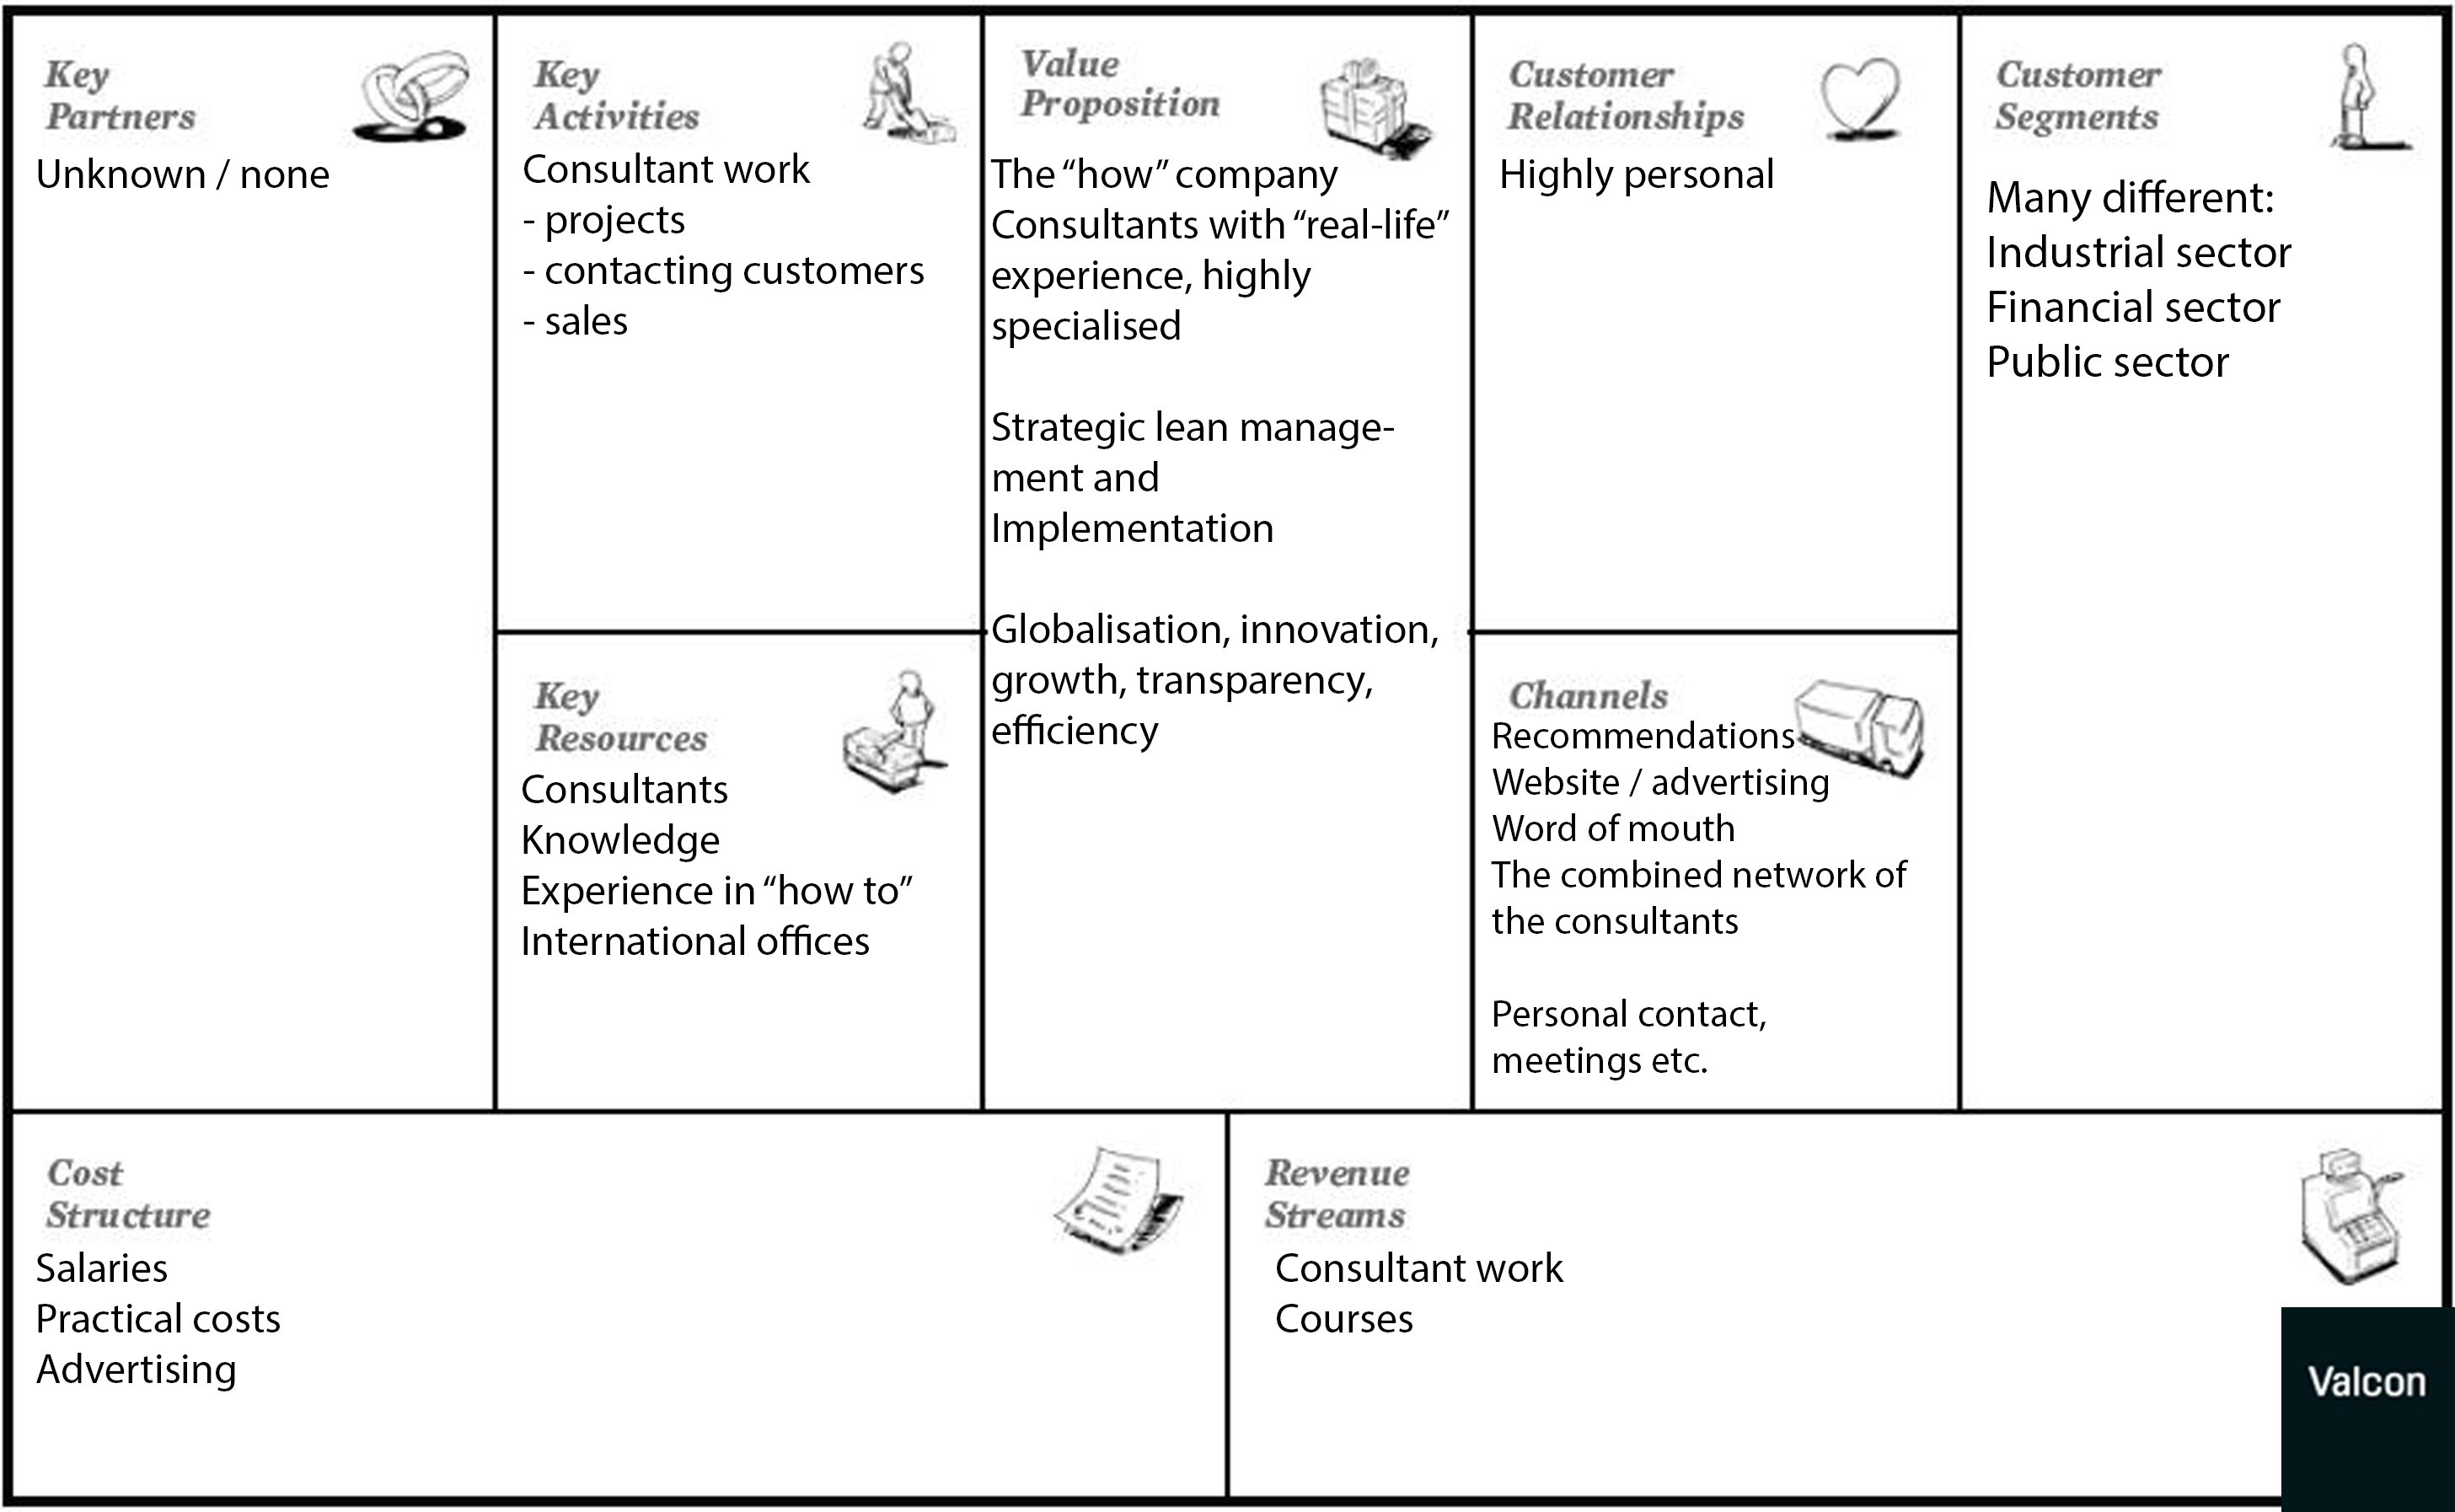
\includegraphics[width=\textwidth]{inline/business-model-canvas.png}
\caption{Valcon's business canvas.}
\label{fig:canvas}
\end{figure}

The Business Canvas gives an overview of Valcon as a whole. In relation to the problem it is important to note that the consultants are key resources for Valcon's business, as they are the ones who generate revenue.
As such it is important that they are able to perform their work effectively as soon as they start working at Valcon. It gives us a good understanding of why the company might value the consultants' time highly. (Sources: Initial meeting with Danni (appendix \ref{app:danni_initiation}), Valcon's homepage. Approved by Danni during inline conclusion meeting (appendix \ref{app:danni_inline}).) (See appendix \ref{app:canvas}.)

We have chosen not to do a canvas for OMT because \todo{Why no OMT canvas?}
\section{Business strategy, IT strategy and key values}
\subsubsection{Business strategy}
We were not able to acquire Valcon's business strategy, as it is not public and Valcon were not interested in sharing it. (Source: appendix \ref{app:business_strategy_refusal}). 
However, we were able to glean some of it through the interviews and meetings:

Valcon is in rapid growth and have a continued focus on keeping this growth as high as possible. 

(Sources: appendix \quoteref{app:danni_initiation}{danni_init_eksplosiv_vekst} and appendix \quoteref{app:danni_initiation}{danni_init_business_strategy_vekst}).

\subsubsection{IT strategy}
Valcon's IT strategy focuses on streamlining IT activities, being cost efficient, outsourcing labor intensive tasks, making work easier for the consultants, few but strong partnerships and choosing off-the-shelf systems instead of customized systems.

See appendix \ref{app:it_strategy} for the original document.

\subsubsection{Company values}
Valcon is guided by four values internally: Integrity, joy, performance, and competence.
Furthermore they value a flat hierarchy.
(Source: appendix \quoteref{app:danni_initiation}{danni_init_firmastruktur}).
\section{Work domains}
The problem involves the following work domains:

\begin{itemize}
\item \emph{OMT and Valcon recruiters} contact and acquire particulars of the new employee. They send this to accounting. \\
(Source: appendix \quoteref{app:danni_initiation}{danni_init_recruiter}).

\item \emph{Accounting} sets the employee up in the economical systems and handles the contract. \\
(Source: appendix \quoteref{app:danni_initiation}{danni_init_accounting}).

\item \emph{IT} sets the employee up in the internal systems, sets up a computer and sends it to him/her, and sometimes sets up a phone and internet connection as well. \\
(Source: appendix \quoteref{app:danni_initiation}{danni_init_IT}).

\item \emph{New employees} are contacted about contract, computer, phone, and internet information. \\
(Sources: appendix \quoteref{app:peter}{peter_stamdata} and \quoteref{app:lisbeth}{lisbeth_kontrakt}).
\end{itemize}

A visual representation of the organization as well as the work domains to investigate can be seen in appendix \ref{app:OrganizationalChart}.
\section{Conclusion}
Part of Valcon's business strategy is to maintain a high growth rate for the company.
A high growth rate means many new employees.
All employments go through Group Support Functions (IT and Accounting).

Since Valcon intends to keep growing, it is relevant to investigate whether the process needs to be optimized or not.
\chapter{In-depth analysis \\ Understanding the problem}
The following chapter will explain our approach to analysing the process, describe the process in some detail and highlight key findings.

\section{Stakeholders}
We have identified the following stakeholders: 
\begin{itemize}
\item Head of IT - Initiator of the project. high power, high interest.
\item IT department - Main recipients of the project. Low power, high interest.
\item Accounting - Recipient of the project. Some power, high interest.
\item HR in Valcon and OMT - Part of the process. Some power, some interest.
\item Recruiters in Valcon and OMT - We may change their work flow. Some power, low interest.
\item Group Operations Director - Head of Accounting, IT and HR. Very high power, low interest.
\end{itemize}
The Group Operations Director has a lot of power, but only low interest, and is a beneficiary, so we chose not to interview him.

For a visual representation, see appendix \ref{app:stakeholder_diagram}.
\section{Process description}
The process starts when a new employee has been hired.
An initiator (often Hanne or Jytte, sometimes other people) contacts accounting with information on the new employee.
A contract has to be formulated and, if there is information missing, the new employee has to be contacted in order to complete their particulars.

The information is entered into QHR and IT is contacted to let them know that a new employee has been hired.
IT then uses the information in QHR to create a new user in AD and give them a mailbox on the Exchange Server, and contacts accounting again with the employee's initials.
Accounting, after receiving the initials, enters the employee's particulars in Maconomy and Bluegarden (or in the case of foreign departments, the relevant salary system for that country).

At the same time IT contacts the new employee about their preferences for phone and internet.
When they have received these from the employee they contact Valcon's communications provider in order to set the new employee up according to their preferences.

Also at the same time, a PC is set up by IT according to the new employee's needs, based on which department they will work for.
Finally information about the handed out gear is recorded in TechAdm.

A visual representation of the process can be found in appendix \ref{app:ProcessChart}
\section{Identified Problems}
\subsection{Results from interviews}
There are several reasons why the current recruitment process needs to be optimized.

\begin{enumerate}
\item The main frustrations in the IT-department are that some recruitments occur with very short notice, and that data occasionally is incomplete.\\
(Appendix \completeref{app:peter} lines \lineref{peter_datamangel}, \lineref{peter_frustration1}, \lineref{peter_frustration2}, and \lineref{peter_frustration3}).
\begin{itemize}
\item The incomplete data for the IT department occurs with recruitments from OMT, while the short notices mainly are rooted in the recruitment of subcontractors in OMT.\\
(Appendix \quoteref{app:peter}{peter_short_notice}).
\item Part of the problem with incomplete data is that the recruiters are not aware of exactly what information is needed in order to set a new employee up correctly.\\
(Appendix \quoteref{app:jytte}{jytte_stamdata}).
\item Valcon employees have a notion that the IT department should be able to handle everything with short notice. Not all IT employees share this opinion.\\
(Appendix \quoteref{app:peter}{peter_klare_IT_bare} and \quoteref{app:hanne_interview}{hanne_snakker_om_IT}).
\end{itemize}

We think that some of the frustration stems from IT not having a standard process for when data is incomplete.

\item The main frustration in Accounting is that it is difficult to get an overview, as employee data is managed in many different systems, and that data is incomplete.\\
(Appendix \quoteref{app:lisbeth}{lisbeth_overblik}).
\begin{itemize}
\item Each employee in the recruitment process maintains their data on the new employees in individual spreadsheets.\\
(Appendix \quoteref{app:lisbeth}{lisbeth_ark}).
\end{itemize}

This is problematic, as responsibility of the current process is difficult to pass on to another accountant.

\item A lot of time is spent communicating information back and forth between Accounting and Recruitment. \\
(Appendix \quoteref{app:lisbeth}{lisbeth_vende_tilbage}).
\begin{itemize}
\item Similarly time is spent communicating information to the IT-department.\\
(Appendix \quoteref{app:lisbeth}{lisbeth_IT}).
\item Accounting and IT want communication to be more standardized. Recruitment finds this problematic because data may be missing at the time of recruitment.\\
(Appendix \quoteref{app:lisbeth}{lisbeth_standardiseret_proces}, \quoteref{app:peter}{peter_standardiseret_proces} and \quoteref{app:hanne_interview}{hanne_ikke_standardiseret_proces}).
\item Forcing standardized communication might put additional pressure on the consultant/manager in charge of the recruitment, which should be avoided.\\
(Source: appendix \quoteref{app:hanne_interview}{hanne_standardised}).
\item At OMT requiring standardized communication might be possible.\\
(Source: appendix \quoteref{app:jytte}{jytte_standardised}).
\end{itemize}

With a common system for keeping the information, problems 2. and 3. could be avoided, as everyone could view the data within that system.

\item Time is spent on routine tasks, such as defining new initials.\\
(Appendix \quoteref{app:peter}{peter_initialer}).

This could possibly be automated.

\item Time is wasted waiting for other IT employees, as IT doesn't have standard processes for communication.\\
(Appendix \quoteref{app:emails}{matias_on_structure}).

This is outside our scope, but should be investigated.
\end{enumerate}

A visual representation of the chain of problems can be found in appendix \ref{app:ProblemChain}.
Note from the interviews can be found in appendix \ref{app:interviews}.

\subsection{The numbers}
\begin{wrapfigure}{r}{0.5\textwidth}
\vspace{-20pt}
\centering
\includegraphics[width=0.45\textwidth]{appendix/total_hires_per_half_year.png}
\label{fig:total_hires_per_half_year}
%\caption{Total number of new hires per half year.}
\end{wrapfigure}
Looking at the number of new hires in Valcon we got an impression of the scope of the problem.
Even though there are some fluctuations there is a trend toward a growth in the number of hires.
This corresponds with the expressed business strategy of growth.
However, the data is not entirely conclusive, as we have only been able to look at the number of new hires within the last 30 months.

Despite the trend toward a growth in the number of hires, the total numbers of hires is still relatively small.
The total hours spend on hires is currently about 190 hours a year.
Even if a solution could cut this down by 25\% it would only save about 47 hours.

A table with all the numbers of new hires can be found in appendix \ref{app:recruitment_data} together with additional graphs.
A full analysis of the time spent on the problem can be found in appendix \ref{app:time_spent_on_the_problem}

\section{Conclusion of In-depth phase}
Optimizing the recruitment process at Valcon is not a simple matter of changing the current process to a more standardized form.
The needs are quite different between OMT and Valcon and the optimized solution needs to take this into account.

Additionally it is not just a matter of introducing a new system to automate the process more than it is today. It is also a matter of making an organisational change, making sure that the recruiters who initiate the process know exactly what information is required for the rest of the process, such that the correct information can be acquired from the beginning and passed on.
\chapter{Innovation \\ Possible solutions}
In this section we will explain our overall vision, describe and analyze our solutions, recommend an implementation strategy and finally make some recommendations for future analysis.

\section{Vision for overall change}
IT and Accounting are frustrated by the recruitment process and feel that time is wasted on it.
Our solutions aim to alleviate these frustrations and reduce the time spent on the process.

Instead of a single solution to the problem, we have decided to look at many small solutions, and recommend implementing many of them.
This is because the Valcon Group is two companies, and solutions that fit OMT do not necessarily fit Valcon Consulting.
We don't want to throw the current process away, but instead want to improve it in small ways to be able to scale with the company growth and possibly save some money.
Finally, we weigh work enjoyment and appreciation highly, as these are important for employee joy, integrity and competence, three of the Valcon Group's key values.

\section{Solutions}
Please refer to appendix \ref{app:solution_propositions} (p. \pageref{app:solution_propositions}) for a complete list of solution propositions.
Each solution contains a description, some positive and negative effects, a financial estimate (refer to appendix \ref{app:cost_benefit_analysis} for the cost/benefit analysis) and a conclusion describing it's suitability.

\subsection{Template for recruitment}
\emph{Description:} Create a template for recruitment so recruiters know what information is required. A template also functions as a checklist, ensuring that the writer knows what information to send.

\emph{Pros:} Could reduce the amount of missing information in the initial email to accounting or IT. 
Also leads to a better defined process.

\emph{Cons:} Requires additional work by recruiter. 
If template is too information heavy, some may ignore it.
Valcon employees dislike forms and rigid processes, so they may ignore it.

\subsubsection{Finance}
This solution would save appr. 6.500 DKK in the first year and appr. 8.000 anually afterwards, including initial costs and maintenance.

\subsubsection{Conclusion} Creating a template for OMT recruitment seems a good idea.
Creating one for Valcon would be a bad idea, as it would take time from management and consultants, but creating one for Hanne might work, as she would be reminded of the information required.

\subsection{Change of attitude toward IT}
\emph{Description:} Change the company attitude toward IT, from the current "they are there to fix my problems" to "they are there if I really need them".
Could be implemented with a small, internal campaign to improve relations to IT, and to make IT feel more appreciated.

\emph{Pros:} May reduce the number of edge cases, as recruiters would be more likely to send recruitment information in early or give warning that a quick recruitment is coming up.
Doesn't require extra time from recruiters.

\emph{Cons:} It would be hard to measure the success of the change - when is an attitude changed?
There might not be a financial gain.

\subsubsection{Finance} 
This solution would probably not save money, but the non-financial benefits are important and the cost is low (appr. 20.000 DKK once.)
Some money may be saved by reducing the amount of edge cases.

\subsubsection{Conclusion} 
We would recommend implementing this change. 
The reduced level of frustration in IT and greater work enjoyment would be worth it.

\subsection{Buffer of computers}
\emph{Description:} Keep 2-3 pre-installed computers ready for use at OMT and at Valcon, for emergencies or very quick recruitments.

\emph{Pros:} Would reduce response times to urgent recruitments.
Also useful if an employee's computer breaks, to reduce downtime.

\emph{Cons:} Needs a little more managing from IT, as
computers will need to be kept updated and ready.
As all computers are not in use, this creates a small overhead.

\subsubsection{Finance} 
This solution has a big initial investment (240.000 DKK) and will not break even unless errors happen.
The money saved comes from employees being able to get back to work quickly after a computer breaks down, or letting new employees start work faster.

\subsubsection{Conclusion}
Whether this solution should be implemented depends on how many errors happen.
We have not been able to get an estimate of how much time is lost due to computer errors or new employees waiting for computers.
As it would increase work enjoyment in IT and help with errors, we would recommend implementing this even with a small financial loss.

\subsection{New HR system}
\emph{Description:} Acquire a new HR system to facilitate communication between accounting, IT, and recruiters.
Valcon is already looking at HR systems.

\emph{Pros:} Recruitment process becomes more standardized, as it always follows the same path.
Information becomes more consistent, as personal spreadsheets are less needed. 
This also safeguards against employees leaving.
Errors are less likely, as number of manual entries of information is reduced.

\emph{Cons:} Costly to implement, requires training of accounting, IT, and recruiter employees.
Also requires maintenance.

\subsubsection{Finance}
We have been unable to make an estimate of the price of a new HR system.
\todo{Maybe we can make this estimate?}

\subsubsection{Conclusion} 
This solution is very necessary, as it is the only way information becomes more consistent.

\subsection{Other small improvements}

Write! \todo{The small improvements need including in the report.}


\section{Implementation}
\todo{do}

\section{Other recommendations}
Need rewriting \todo{Is this section good? Is it relevant?}

\subsection{Analyze OMT process}
Conduct an analysis of whether the OMT process can be improved so they know further in advance who and when someone is needed, so the number of urgent cases can be reduced.

\subsection{Further automation of install process}
The install process is very time consuming, and is a candidate for automation.
Looking into whether more of it could be automated could save time.



\appendix
\chapter{Glossary}
Valcon Group	=	The company we are working with \\
Valcon 			= 	Part of the Valcon Group, based around consultants \\
OMT 			=	Odense Maritime Technology. Part of the Valcon Group, based around designing ships \\
Particulars 	=	The core data of a person (name, address and more) \\
Lotus Notes		=	Platform at which QHR and TechAdm is hosted	\\
QHR				=	HR platform used to store information about new employees	\\
AD				=	Active directory. Platform used to generate and organize information in the Valcon portal, user control and permissions	\\
TechAdm			=	Platform used to store information about rented hardware	\\
Maconomy		=	Platform used to administrate invoices	\\
Exchange		=	Platform used to administrate the Valcon mail system	\\
BlueGarden		=	Platform used to administrate salaries in Valcon Denmark	\\
\chapter{Project Agreement}
\section{Premise}

\subsection{Background}
In Valcon, the process of registering new employees is characterized by loose organization. This is a problem, as the company is growing quickly and many employees are recruited, and specialists are recruited for short periods of time. We have been asked to research this process and explore possible solutions, and finally to write a business case explaining the benefits and drawbacks of different solutions.

\subsection{Assignment and Objective}
The objective of the project is to research the process of registering new employees. HR departments in both OMT and Valcon collect information on the new employee and send this to either an accountant or the IT department, depending on what they need done first. This creates an unnecessary need for communication between the IT department and the accountant, which might be avoided if the process was standardized. The accountant enters financial and personal information into a system (QHR), which the IT department then uses to send a computer, setup internet connection and phone accounts, and enter the employee into the central system (AD). To further understand the current situation, the project group will conduct an ethnographic analysis of the process, in an attempt to discover parts of the process that could be effectivised, and look at ways to do so.

\subsection{Financial framework}
There will be no money involved in the project.
The resulting report of the project may be used freely by Valcon.

\subsection{Critical factors}
\textbf{Success factors:}
The solutions proposed should reduce the time, complexity and effort it takes to enter a new employee into the system.
The Business Case provided by the group must, regardless of the solutions proposed, be useable as documentation for the existence of the problem.
The solution proposed must still make use of the Active Directory which Valcon uses for managing their IT structure.
\textbf{Critical preconditions:}
We need to be able to get the time needed from the resources mentioned below.

\section{Organization}
\subsection{Project organization}
The project organization consists of two groups. The project group at ITU consists of Michael Frikke Madsen, Jonas Kastberg Hinrichsen, Martin Juul Petersen, Jakob Ambeck Vase, and Jakob Merrild. They report to Danni Jensen at Valcon.

\subsection{Resources}
The time of the project group.
3 meetings (with a 4th optional one) with Danni Jensen of appr. 1 hour each.
One or two interviews with each key employee in the process (Lisbeth, Peter, Mathias, HR) of appr. 30 min. each.
Open doors, for observing the work practises involved in the process.

\subsection{Stakeholders}
Danni Jensen
Lisbeth Justesen
The IT department of Valcon
HR departments of OMT and Valcon

\subsection{Agreements}
The following agreements were made:
The project group can conduct observations of public areas at Valcon without prior notice.
In order to conduct interviews with and observations of individuals, an agreement must be made with Danni Jensen, who must authorize the project group to initiate contact with the person to be interviewed. 
After the initial contact has been made, the project group is free to contact the person directly in order to make an appointment.

\section{Method}
\subsection{Overall Approach}
The overall approach to the project will be using the MUST method. The MUST method consists of the following four phases:
Initiation phase, where we agree on the problem and a contract
In-Line analysis, where the project group will align the project’s goals with the company’s IT and business strategy
In-depth analysis, where the project group will observe and document the relevant work practices
Innovation phase, where solutions will be investigated and optionally presented

\subsection{Plan}
\begin{itemize}
\item[13/10] - End of In-Line phase.
\item[15/10] - Meeting after In-Line and before In-Depth phases.
\item[10/11] - End of In-Depth phase.
\item[14/11] - Meeting after In-Depth and before Innovation phases.
\item[4/12] - End of Innovation phase
\item[Before] 17/12 - Delivery of Business Case
\item[??] - Optional meeting after Innovation phase.
\end{itemize}

\subsection{Signatures}
\chapter{Problem Statement}
\label{app:problem_statement}
How can the Valcon Group save time and reduce frustration in the IT and Accounting departments by improving the process of new employee registration?
\\\\
Specifically:
\begin{itemize}
\item How can they reduce redundant work?
\item How can they automize routine tasks?
\item How can they reduce the amount of cases not following the standardized process, or refit the standardized process to accomodate the open structure of the company?
\end{itemize}

The following requirements need to be fulfilled for the project to be considered a success:
\begin{itemize}
\item
We must document the process to prove that there is a problem.
\begin{itemize}
\item If we prove that there is a problem, this requirement is fulfilled.
\end{itemize} 
\item
Having a standardized process reduces frustration and saves time, therefore communication should go through accounting every time, or standard process should be changed to allow for multiple paths.
\begin{itemize}
\item
Measure the amount of tasks currently not following standard process (mean/month)
\item
After implementation, measure the amount of tasks not following standard process (mean/month)
\item
If the number of tasks not following standard process after implementation is reduced by 50\%, this requirement is fulfilled.
\end{itemize}
\item
Tasks that could be automated, should be.
\begin{itemize}
\item
Look at the process, find all the tasks that could be automated and the ones that already are, make a list stating whether a task is manual or automated, and whether it must be manual or could be automated.
\item
After implementation, look at the list and compare the number of “could be automated” tasks to current process.
\item
If 50\% of the tasks that were previously not automated, but could be, are now automated, this requirement is fulfilled.
\end{itemize}
\item
The current speed of the process must be maintained or improved.
\begin{itemize}
\item
Measure the current mean time from first mail to accounting or IT, to employee is registered and IT tasks are done before and after implementation.
\item
If this time is the same or (preferably) faster, this requirement is fulfilled.
\end{itemize}
\end{itemize}
\chapter{Valcon environment}
\label{app:valcon_environment}
Valcon operates within an competitive environment where image and contacts are key. 
There's a great need for experienced and knowledgeable consultants but there's also a lot of competition in the field.
Not because there are a lot of competitors within the fields that Valcon works in, but rather because the competitors are the same every time.
This means they know each other and know exactly what kind of prices and quality the opposing firms will bring.
Due to this, Valcon's business strategy has been to hire the best and brightest employees and accept the fact that they're unable to be the cheapest organisation to hire.

They sell themselves mainly on knowledge and quality, rather than on price and pride themselves on being a company capable of the entire consultation process, from analysis to implementation.

They refer to themselves as the 'how' company, as they are often employed in projects where a competing consultation firm has been hired to write the analysis report and figure out 'what' to do. 
Valcon are then employed to conclude the project by implementing the solution.

Valcon's biggest threat is losing their consultants.
Consultants are drawn towards new and exciting opportunities, while working for the same company for a long time gets increasingly stale.
This means that sooner or later a consultant will grow tired of the current challenges he's facing and move on to another company.
\chapter{OMT environment}
\label{app:OMT_environment}
OMT operates within an environment where they aren't facing a lot of competition. 
There aren't many firms designing war ships, and this places OMT in a favorable position.

There aren't many ship designers with experience on war ships, so when OMT needs employees there aren't many candidates, and most of them are already employed elsewhere.
Because of this, OMT hires a lot of their workforce within other ship design companies.
Since these companies work in other fields than OMT, they don't mind OMT subcontracting their employees, as it benefits them as well. 

For references, see \completeref{app:danni_initiation} and \completeref{app:danni_inline}
\chapter{Valcon Business Canvas}
\label{app:canvas}

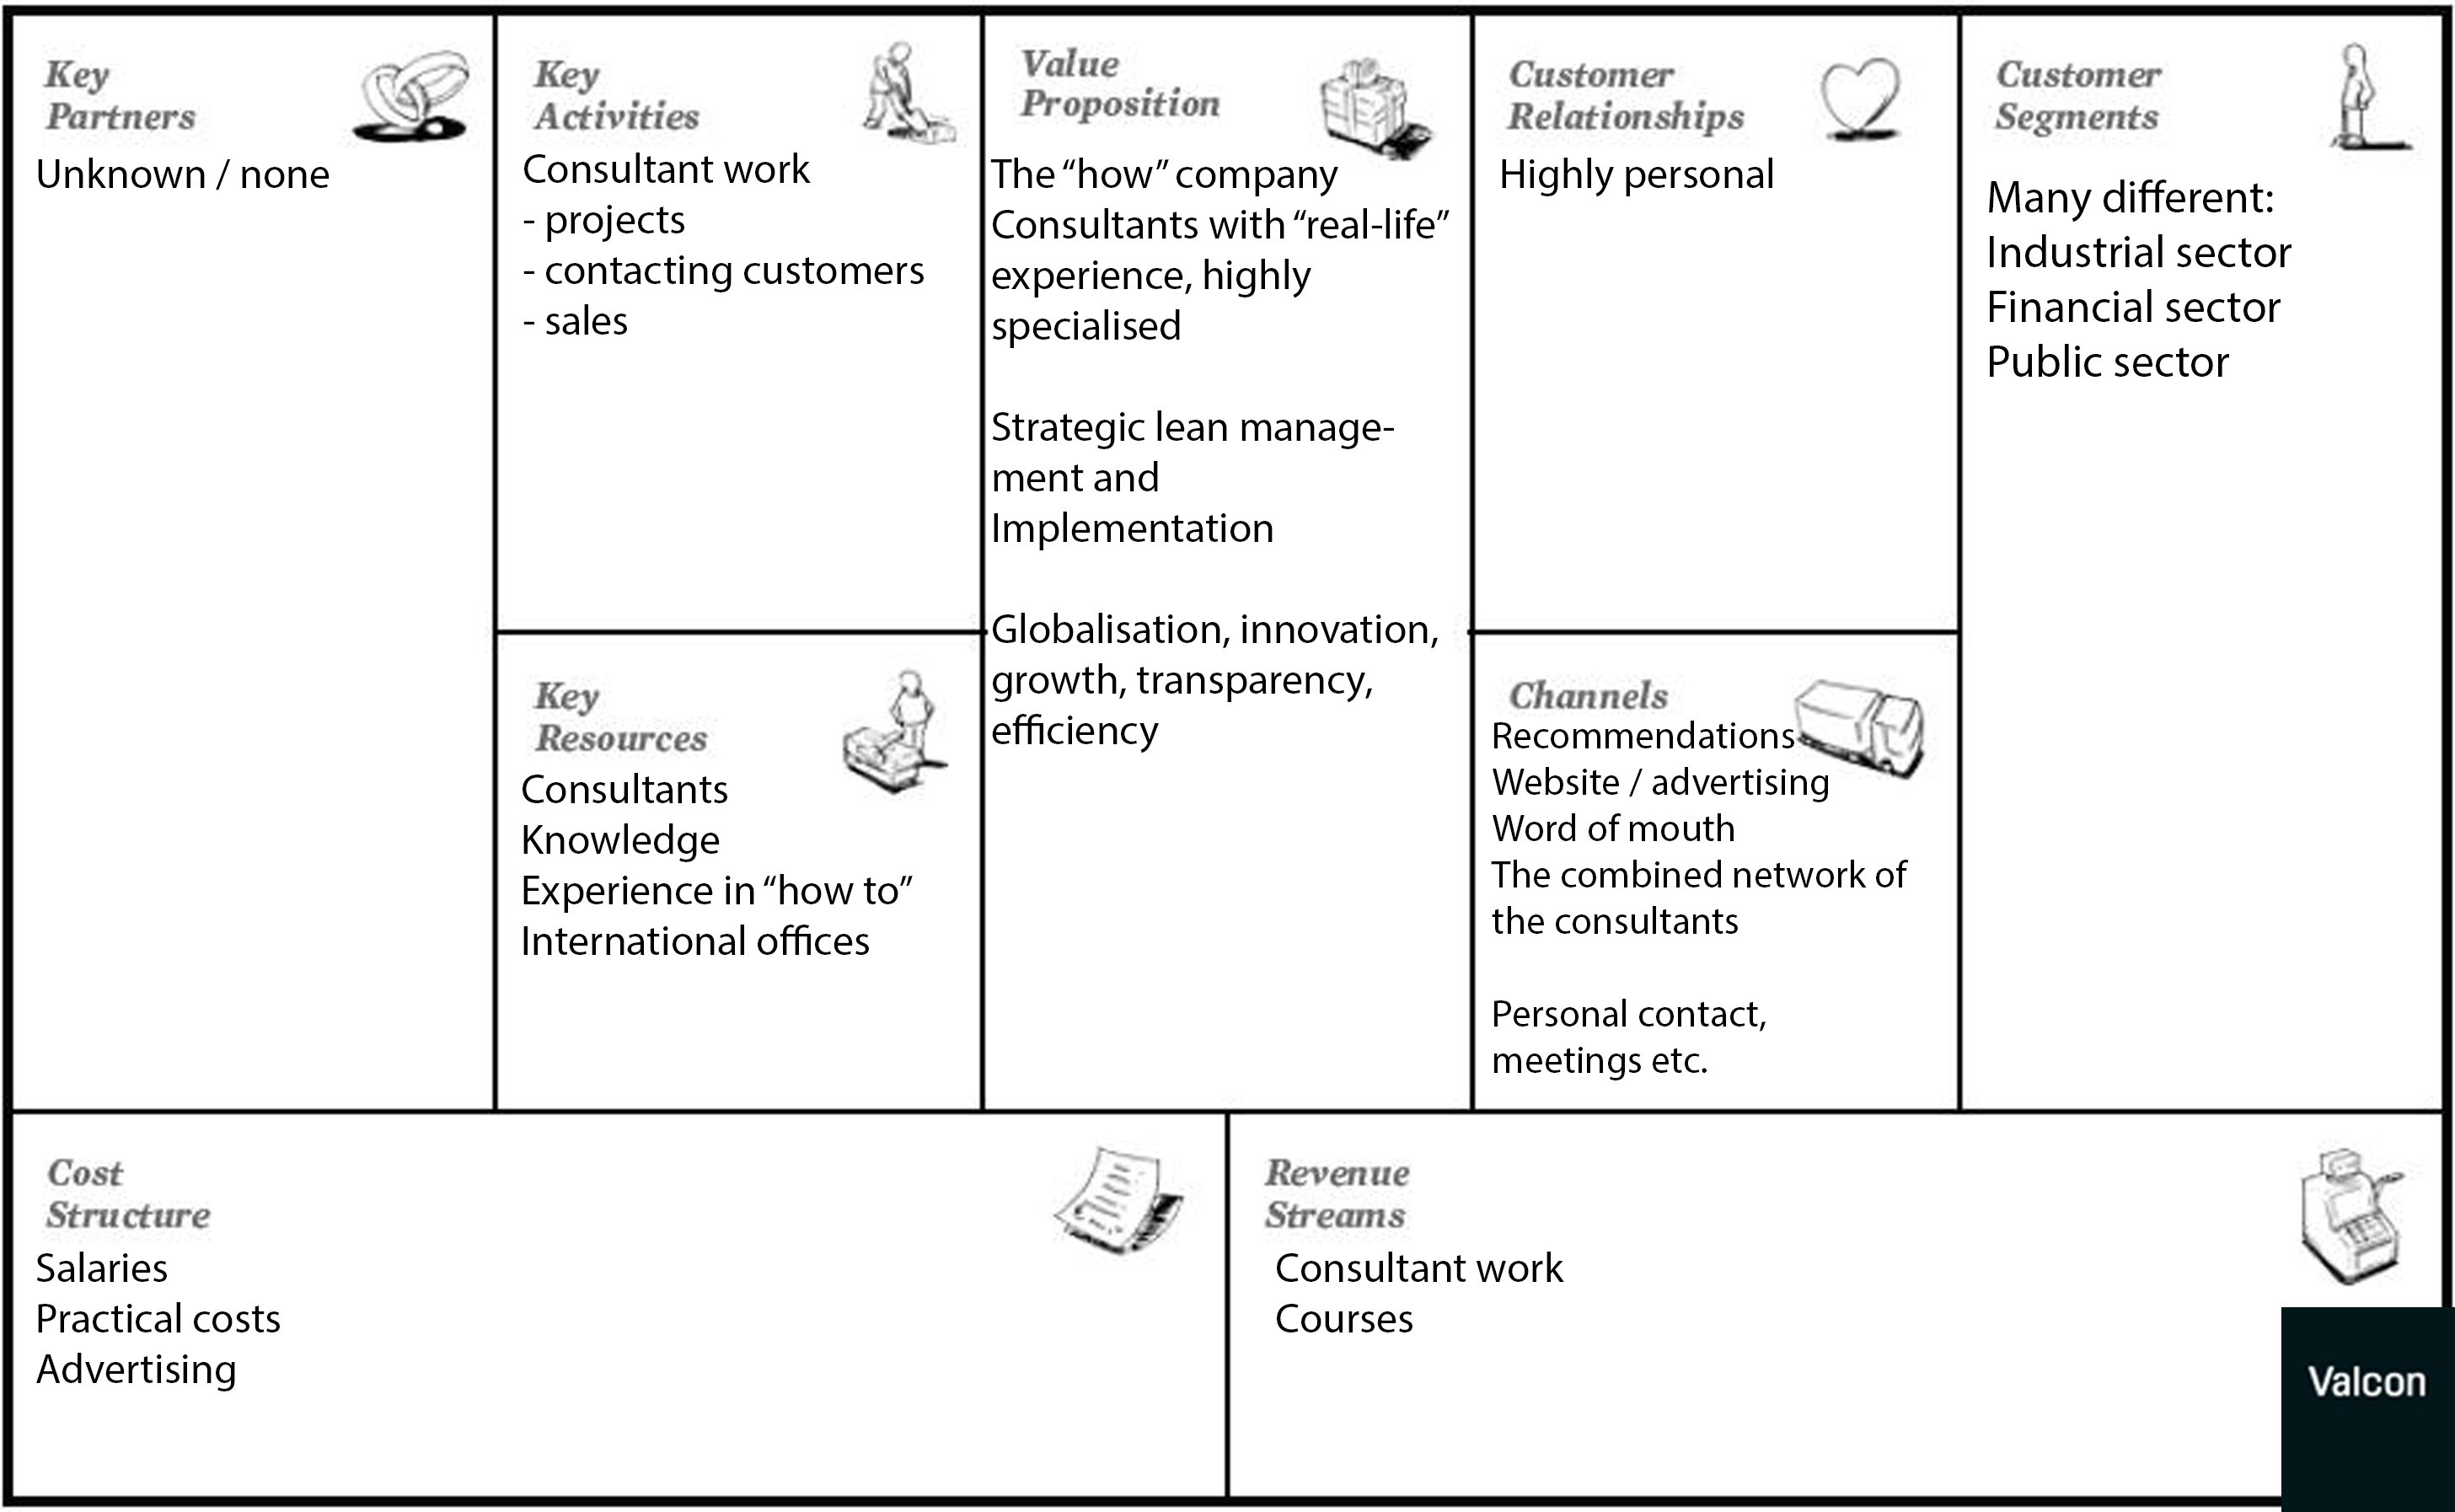
\includegraphics[angle=90,height=475pt]{inline/business-model-canvas.png}

The business canvas gives an overview of Valcon as a business - what services they provide, what their key resources are and so on.
We constructed the canvas primarily from information from the Valcon website, along with information from initial interviews with the IT Manager of the company.
The canvas was later presented to the IT Manager, and then refined slightly from his feedback.
\includepdf[pages={1-2},pagecommand=\chapter{Valcon's IT strategy},scale=0.75,nup=1x2]{appendix/it_strategy.pdf}
\label{app:it_strategy}
\includepdf[pages={3-},scale=0.75,nup=1x2]{appendix/it_strategy.pdf}
\chapter{Organizational Chart}
\label{app:OrganizationalChart}
\includegraphics[angle=90,height=475pt]{appendix/organizational_chart.png}

\chapter{Process Chart}
\label{app:ProcessChart}

This chart visualises the process.
If two arrows point to one square, both actions must be completed before continuing with the next task. \todo{Please write this text inside the diagram, so it looks better.} \todo{Please explain the orange arrows (also inside the diagram)} \todo{Consider writing less convoluted, so the meaning is easier to understand.}

\includegraphics[scale=0.325]{appendix/ProcessFlowChart.png}
\chapter{Problem Chain}
\label{app:ProblemChain}

Problem chain visualizing the origin of each problem.
The origin reason of a problem are the ones that are not affiliated with a problem in another work area. \todo{Forstår ikke?}
These problems are the most important to look into.

\includegraphics[scale=0.75]{appendix/ProblemChain.png}
\chapter{Solution propositions}
\label{app:solution_propositions}
\section{List of solution propositions}
\begin{enumerate}
\item Software that does it all
\item Template for recruitment
\item Change of attitude toward IT
\item Buffer of ready computers
\item Increase IT staff size
\item New HR-system
\item Help-program for finding initials and reading templates
	\item Other small improvements
	\begin{enumerate}
	\item Phone and internet paper in contract letter
	\item "Unkown department" in IT-systems
	\item Mail from OMT when recruitment is assured, but data is not yet available
	\end{enumerate}
\end{enumerate}

\section{Explanation of solution propositions}
\subsection{Software that does it all}
\emph{Description:} This proposal is for a piece of software that can encompass all the requirements of every employee in the company. Lotus Notes had this status once, but many disliked it.

\emph{Origin:}
When interviewing the accounting department it was noted that such a system would help out with a lot of the prevalent tasks.
(Source: appendix \quoteref{app:lisbeth}{lisbeth_system})

\noindent \emph{Pros:} Only one place for information, easy to manage.

\noindent \emph{Cons:} Very expensive, very hard to accomodate everybody.

\emph {Verdict:}
Not suitable. The solution is in direct opposition to the business strategy of the company, as it would require a large amount of concrete templates, training and time on behalf of the consultants.

\subsection{Template for recruitment}
\emph{Description:} When a new recruitment process starts, instead of a mail being sent with the information, a template is used to ensure that no information is missing.

\emph{Origin:}
In various interviews it was mentioned how lack of information damaged the recruitment process a lot, by increasing the overall work load required.
(Source: appendix \quoteref{app:lisbeth}{lisbeth_vende_tilbage} and appendix \quoteref{app:peter}{peter_information})

\noindent \emph{Pros:} No information missing means no need to contact employee more than once, saving time.

\noindent \emph{Cons:} Will put more work on recruiter, and Hanne stated that employees at Valcon dislike templates, so they won't use them.

\emph{Verdict:}
Partially suitable. The solution is in direct opposition with the Valcon business strategy, and thus we would not recommend it. However, based on interviews with the OMT partition of the company, templates would be possible for recruitments on their end. Thus we recommend it for the OMT group.

\subsection{Change of attitude toward IT}
\emph{Description:} Change the general attitude toward IT. Currently, IT is generally regarded as a department that just solves whatever problem one might have. Changing this attitude to better reflect the level of stress in IT could have benefits.

\emph{Origin}
When interviewing the IT department there was a notion that the company did not realise the amount of effort put into the work of the IT deparment, nor did most understand how complicating it was if recruitment requests were admitted with little to no spare time.
(Source: appendix \quoteref{app:peter}{peter_frustration3})

The other interviews backed up this notion, as they seemed to not know the implications of the IT departments work processes.
(Source: appendix \quoteref{app:lisbeth}{hanne_omIT} and appendix \quoteref{app:hanne_interview}{hanne_losningomIT})

\noindent \emph{Pros:} If people are more aware of how the IT department functions, they are more likely to be considerate. We think it would reduce the number of urgent cases and make IT more happy. Doesn't increase workload of consultants or management.

\noindent \emph{Cons:} Hard to implement, hard to measure.

\emph{Verdict}
Suitable. In order to maintain a high satisfaction for all employees, it is important that everyone understands each others work loads, and how it is increased under certain conditions. It would be easily achieved through generic information channels in the company.

\subsection{Buffer of ready computers}
\emph{Description:} Have a few number of computers installed and ready for use at Valcon and OMT.

\emph{Origin:}
In various interviews it was mentioned how this solution could ease the overall process, as it can deal with the situation of a critical recruitment.
(Sources: \quoteref{app:hanne_interview}{hanne_buffer} and \quoteref{app:jytte}{jytte_buffer})

\noindent \emph{Pros:} Better response times to urgent recruitments. Useful if an employee's computer breaks at a critical time.

\noindent \emph{Cons:} Needs a little more managing from IT, and maybe a full time IT employee at OMT. Computers will need to be updated. Resources not in use.

\emph{Verdict:}
Suitable. Having a buffer of computers would increase overall budget, but would solve many issues related to the recruitment process.

\subsection{Increase IT staff size}
\emph{Description:} Increase the IT staff size to increase throughput.

\emph{Origin:}
Baseline solution

\noindent \emph{Pros:} Makes IT capable of doing more.

\noindent \emph{Cons:} Expensive, and management increases.

\emph{Verdict:}
Not suitable. Simply increasing the size of the IT staff to accomodate demand is not a proper solution, as it would not increase the amount of capable workers. This is due to increased management of the IT department. The issues faced in the process cannot be reduced by simply having more employees working on it.

\subsection{New HR system}
\emph{Description:} Implement a new HR system for communication between accounting and employers.

Valcon are already looking at new HR systems.

\emph{Origin:}
In the interview with accounting, it was mentioned how the current HR system was deprecated, and not very user-friendly.
(\quoteref{app:lisbeth}{lisbeth_HR})
A new HR system would help the process in a way, that information has to be typed in fewer times.

\noindent \emph{Pros:} Process becomes more standardized and information more consistent. Copying data fewer times reduces probability of errors.

\noindent \emph{Cons:} Costly and requires training.

\emph{Verdict:}
Suitable. A new HR system would affect the company positively in relation to their business strategy.

\subsection{Help-program for finding initials and reading templates}
\emph{Description:} 
Write a small program that can read the template proposed above and enter the information into the IT systems.
Also able to propose initials for employees, and check whether the exchange mailbox has been used before.
Would reduce workload for IT and introduce fewer errors, but would require some maintenance and some time initially.

\emph{Origin:}
When interviewing the IT department it was mentioned how a tedious task it was to make up new initials. Since the making of initials are based on certain rules it is possible to generate them automatically. Furthermore they have to input data in various databases, as well as updating possible deprecated data.
(Sources: \quoteref{app:peter}{peter_initialer} and \quoteref{app:peter}{peter_old_employees})

\noindent \emph{Pros:} 
Less time used to making initials. Reduction of tedious tasks that must be conducted often.
Less time used on inputting data, reduction of possible typing errors.

\noindent \emph{Cons:} 
Generated initials might form unsuitable words, and the process has to be overridden by the employee.
System might be insufficient and not be capable of handling deprecated data correctly. 

\emph{Verdict:}
Partially suitable. The initials systems can be implement fairly easy. It can be taken into account that it must be possible to manually input initials if the generated initials are not sufficient.
The automated system will be too difficult to manage.

\subsection{Other small improvements}
\begin{itemize}
	\item Phone and internet paper in contract letter\\
	
			Put a paper in the contract letter sent to new employees, asking for their internet and phone preferences. Give it to IT upon return. Would help reduce missing data for new employees, and save time in IT.
			(Source: \quoteref{app:peter}{peter_blanket})			
	
	\item "Unkown department" in IT-systems\\
	
			Create a department for unknown departments in the IT systems, possibly both for Valcon and OMT, and create a process for managing it.
			Would remove the department requirement from IT, allowing for quicker recruitment.
			(Source: \quoteref{app:peter}{peter_datamangel})
			
	\item Mail from OMT when recruitment is assured, but data is not yet available\\
	
			Have OMT write a mail to IT when they know they will hire an employee soon, but don't have the data yet, so IT can plan accordingly.
			Would reduce stress, but increase planning for OMT.
\end{itemize}
\chapter{Cost/benefit analysis}
\label{app:cost_benefit_analysis}
These calculations are based on the recruitment and resignation data sheet in appendix \ref{app:recruitment_data}.

\section{Standard process and edge cases}
\begin{itemize}
\item In 2012/13, 118 persons were hired or subcontracted.
\item In 2013/14, 154 persons were hired or subcontracted.
\item In 2014/15, 80 persons have been hired or subcontracted so far.
\end{itemize}
These numbers show how many computers have been made ready by year.
\emph{There is a small increase in the number of computers being readied (30\% in 2013 and 4\% in 2014).}

\subsubsection{Time spent on computers and data entering}
Peter gave an estimate for how long it took him to set up a computer and enter data into the system, 45 minutes (appendix \ref{app:estimat_peter}). (We realize Peter may be wrong about this. We haven't been able to observe the process, but we still think the calculations are useful.)

This means, that Peter has used 88.5 hours in 2012/13, 115.5 hours in 2013/14, and 60 hours in 2014/15 so far on computer setup and data entering.

With less than 150 hours used every year, \emph{this is not a problem where a solution could save a lot of money.}

\subsubsection{Time spent on other things related to recruitment}
Peter uses time on gathering information on telephone and internet connection preferences from the new employees, appr. 10 minutes every time.
This is only on the Danish recruitments, and not on subcontractors.

Furthermore, he uses time on Danish resignations, both subcontractors and hires, appr. 15 minutes each.
(We realize Peter may be wrong about these. We haven't been able to observe the process, but we still think the calculations are useful.)

Here follows the total amount of time spent on recruitments and resignations each year (barring edge cases).
\begin{itemize}
\item 2012/13 - 111 hours.
\item 2013/14 - 148 hours.
\item 2014/15 - 75 hours so far. (Half the year has passed, so a reasonable estimate is that he will use 150 hours total.)
\end{itemize}

As long as there are few edge cases, \emph{the time spent is not a problem.}

\subsubsection{Edge cases}
We haven't been able to get any numbers on the amount of edge cases in the process.

This is problematic, as our main focus is documenting that there is a problem, and the amount of time used without edge cases is small.

And even when edge cases happen, as the process doesn't change, \emph{the time spent doesn't increase, only the level of stress in the IT department.}

\subsubsection{Benefits to improving the process}
There are some benefits to changing the recruitment setup process.

Currently, IT and accounting are both stressed by the process.
By improving the process, the work enjoyment could improve.

Finally, improving the process can speed up response times on support and recruitment from IT and on recruitment in accounting.

\subsubsection{Conclusion of process analysis}
There is little financial gain in changing the recruitment setup process.

The benefits, however, are important and in line with the Valcon's employee values.

So the solutions we propose must be without or with very little cost.

\section{Cost/benefit of solutions}
In this section, we look at the costs of each of our proposed solutions and write a few benefits.
We will not look at the new HR system, as Valcon is already working on it and we do not know enough about the system to correctly estimate costs and benefits.

\subsubsection{Software that does it all}
\begin{itemize}
\item \emph{Costs} - Very high. (\textgreater 1.000.000 DKK)
\item \emph{Benefits} - Accounting and IT would be happy, as all data would have to only be entered once. But consultants would be less so, as their work would be slowed down by data entering and a heavy program. (Lower income.)
\item \emph{Conclusion} - This investment would never break even.
\end{itemize}

\subsubsection{Template for recruitment}
\begin{itemize}
\item \emph{Costs} - Three hours for creating the template, an hour every six months to keep it up to date. (500 * 3 = 1500 DKK initially, 500 * 2 = 1000 DKK anually.)
\item \emph{Benefits} - Lisbeth saves time, as data isn't missing, but Hanne and Jytte spend a little more time gathering the information. All three save time as less communication between them is needed. (Lisbeth saves appr. 10 minutes per recruitment, Hanne goes even, Jytte goes even.) (Minutes saved * number of recruitals anually / 60 = hours saved anually = 10 * 180 / 60 = 30 hours saved anually = 9000 DKK saved anually (assuming 300 DKK/hour))
\item \emph{Conclusion} - This investment would break even in the first year, even saving 6500 DKK, and would save 8000 DKK anually afterwards.
\end{itemize}

\subsubsection{Change of attitude toward IT}
\begin{itemize}
\item \emph{Costs} - A small campaign to change company attitude might cost appr. 20.000 DKK (Two days work for a designer, printing posters, sending emails, lost time for consultants).
\item \emph{Benefits} - Better communication with IT. We cannot see any financial gain. Would reduce stress in IT and make IT feel more appreciated.
\item \emph{Conclusion} - Won't break even, but the non-financial benefits are important.
\end{itemize}

\subsubsection{Buffer of ready computers}
\begin{itemize}
	\item \emph{Costs} - 240.000 DKK initially (20.000 DKK * 12 computers). Appr. 1.200 DKK anually for maintenance (8 hours work for a student-helper, 150 DKK per hour pay.)
	\item \emph{Benefits} - Shorter response times from IT, less stress in IT. Time saved in IT as the computers can be created at the same time. (New employees can start work earlier in quick cases means money saved) (96 hours saved by student helpers anually = 14.400 DKK saved anually, maybe some more from new employees starting early.)
	\item \emph{Conclusion} - Will break even after less than 18 years. Less stress in IT and better response times make it worth it. \todo{net present value?}
\end{itemize}

\subsubsection{Increase IT staff size}
\begin{itemize}
	\item \emph{Costs} - 1.000.000 DKK appr.
	\item \emph{Benefits} - Won't save money. Less stress in IT.
	\item \emph{Conclusion} - This is throwing money at the problem.
\end{itemize}

\subsubsection{New HR-system}
We won't describe this here, as Valcon is already working on it.

\subsubsection{Help-program for finding initials and reading templates}
\begin{itemize}
	\item \emph{Costs} - Writing the program and maintaining it will cost a programmer 5 days initially, and then 1-2 days anually. (12000 DKK initially, then 4800 DKK anually, assuming 300 DKK / hour.)
	\item \emph{Benefits} - Less time spent on entering data, less errors, less stress for IT. (5 minutes * 156 recruitments / 60 * 300 DKK /hour = 3900 saved anually)
	\item \emph{Conclusion} - This won't break even. Should only be implemented to make Peter happier (which might be worth it).
\end{itemize}

\subsubsection{Other small improvements}
\begin{itemize}
	\item \emph{Costs} - These are all free or have very low costs (below 500 DKK over 5 years)
	\item \emph{Benefits} - The benefits are mainly time saved for IT and accounting, except in the case of the mail from OMT, which would help reduce stress.
	\item \emph{Conclusion} - All three of these save a little money or increase work enjoyment slightly for IT and/or accounting.
\end{itemize}
\includepdf[pages={-},scale=0.75,nup=1x2,pagecommand=\chapter{Recruitment data}]{appendix/recruitment_data.pdf}
\label{app:recruitment_data}
\chapter{SWOT analysis}
\begin{figure}[!htp]
\noindent
\includegraphics[scale=0.75]{appendix/SWOT.png}
\end{figure}
\chapter{Meetings}
\section{Initial meeting with Danni}
\label{app:danni_initiation}

\subsection{Summary}

The problem is defined as the recruitment process, the stress undergone during it, the amount of time it takes and how information is managed during. Many different systems are used, and they must all receive data manually.
The process is not uniquely defined as it, in rare cases, must be done quickly, and thus the standardized procedure is not followed. This is mainly a problem for new OMT employees.

Valcon is already working on a new HR system to improve the way information is managed. Danni recommends a solution that automises as much of the process as possible, to avoid human errors in insertion of new data.

Dannis goal for the project is to get a report that document that there is in fact a problem.

Valcons main business strategy is growth.
Their key values are that happiness and integrity is ensured for all employees. Furthermore, their consultants should be deserved as little as possible.

\subsection{Minutes by Jonas Kastberg}
Introduktion:

Der bliver introduceret af de forskellige parter.
Danni er en gamer type
Vase er far
Jonas er der bare
Martin er også gamer
Merrild er også gamer
Michael arbejder her

Præsentation af vores projekt:
Vi skal lave en etnografisk undersøgelse
	- Det er spacy
Vi har brug for 2 møder senere på året
	- Det er intet problem
Der afleveres rapport d. 17 december
Der skal laves en underskrift



Danni: Hvor mange timer skal der bruges herude
Os: Det ved vi ikke
Jakob: evt. en 3 dage herude
Danni: Lisbeth kan være rigtig svær at få tid hos
Danni: Så længe i finder interessenterne kan jeg godt "spearheade"


Introduktion af Valcon:
Danni startede for 5 år siden
Eksplosiv vækst lige siden

IT og accounting vokser ikke meget iforhold til alt andet.
Dette besværliggører hyring af nye medarbejdere til Valcon og OMT
Lisbeth har ingen tid
Det er en meget konservativ kultur i firmaet
Problemet: Hvordan forbedrer man problemet uden at støde nogen i den kultur der allerede er.
Der er allerede en proces, men hvor automatiseres den.

Problemet: Processen skal identificeres, automatiseres og effektiviseres.

Efaring: Kultur og Proces hænger sammen

Afklaring af MUST:
MUST forklares, hver enkelt fase introduceres.
Ingen afklaring af Steering Comittee


Vores forståelse af problemet:
Der er en medarbejder der ansættes, og det kan tage lang tid.
	- Det er mere kompliceret at ansætte en medarbejde end som så.
	- Problemet ligger i hvordan arbejdet kan påbegyndes inden hyringsprocessen er færdigt processed
	- Lisbeth er bottleneck, da hun er den eneste der kan udføre processen
	- Der kan også være flere interressenter, Jytte og Niels hos OMT.
	- Problemet hersker hovedsageligt hos OMT.

Hvem er stakeholders
	- Danni (enighed)
	- Accoutning (Uenighed, foruden lisbeth)
	- Løn er som regel en bottleneck i firmaer

HR-afdelingen
	- Der er to HR medarbejdere, Bjarke og Hanne
	- Der et to medarbejder typer: Stationære og mobile

Nuværende løsning på problemet:
	- Igang med er HR system der kan bygges oven på det nuværende IT problem
	- Deres ERP (fakturering system) er 4 versioner gammelt (der benyttes Maconomy)
	- Evt. problem, streamlining af ERP Systemet. (java skal holdes på samme version for individuelle pc'er, da det ellers ikke understøtter maconomy)

Hvordan ser Danni processen:
	- Valcon melder ind til Lisbeth med en masse personlige oplysninger for ny medarbejder
	- Lisbeth putter det ind i systemet. (QHR, Lotus Notes egen udviklet system)
	- Andre grupper kan tjekke QHR for nye medlemmer.
		- Sekretariatet kigger derinde for at sende blomster og andre bløde ting (Vase likes)
		- IT tjekker og opretter brugeren i AD.
		- IT sender pc og andet til den nye bruger.
	- AD opretter brugeren på knowledge portalen.
	- AD Opretter brugeren på Lync
	- AD opretter mailgrupper til brugeren.
	- AD sætter brugeren i en sikkerhedsgruppe
	- IT opretter en mailbox til brugeren.

Eventuel løsning:
	- Automatiseret løsning for at Lisbeth kan godkende og så ryger det bare ind i QHR
	- QHR skal selv informere om at der en ny medarbejder.


Pipeline for at analysere arbejdspladsen:
	- Vi kan godt komme herud.
	- For kontakt med specialpersoner, kontakt med Danni for authorisation
	- Pipeline:
		- Skriv til Danni med hvem vi vil snakke med og om hvad
		- Danni skriver videre til personen og godkender os.
		- Vi skriver personligt til personen og aftaler tid og sted.

Motivationsfaktoren:
	- Vores sucess (ikke godt)
	- Hvis firmaet kan modtage en rapport der kan give en overbevisende forklaring om at der er et problem, og at det kan løses.


Firmastruktur:
	- Fire medarbejderværdier
		- Integritet
		- Glæde
		- Performance
		- Kompetence
	- Meget flad hierakistruktur


Business Strategy / IT Stategy:
	- Business Strategy = vækst
	- 

\subsection{Minutes by Michael Madsen}


\section{Meeting with Danni after in-line phase}
\label{app:danni_inline}
\begin{linenumbers*}
\subsection{Summary}
During the interview, we show Danni the progress we've made and what we've come up with. 
He mentions that the size of Valcon is both a boon and a bane and explains Valcon's situation in the market and how they stay in the competition despite not being the biggest firm. 
Valcon are good at being with a project from initial to implementation and the projects they put out offers on don't see a lot of competition, so they generally know who they're competing with. 
OMT's choice of working with subcontractors is a conscious decision as it's part of a strategy for the company.

\subsection{Minutes by Martin}
Michael: Hvad er vores forståelse af Valcon og hvordan vores forståelse af processen ser ud
Vi viser vores canvas frem og forklarer hvad det går ud på og hvad vi har skrevet
Danny foreslår at vi skriver ‘the how company’ på, det ville Poul være glad for

Michael: Vi har ikke fundet noget specifikt segment for Valcon\\
Danny: Der er også medico og rejseselskaber/flyselskaber. Det man kan sige er at public sector ihvertfald ikke er den største, det er industry/medico hvis man ser bort fra skibsdesign. Han syntes vi skal specificere at det er i 'no particular order' eller rykke public sector nederst ihvertfald.

Michael: [Det her er de] channels [vi har kigget på]\\
Danny: Relationship building er også en ting, dem der arbejder her ude har en kæmpe kontakt bog på 3500 kontakter som de kan hive på.

Michael: Key activities + key resourcer\\
Danny: I kan inkludere 'experience in how to' under key resources

Michael: Value propositions\\
Merrild: De der Kurser Valcon holder, er det substant?
Danny: Nej, det meste af det er udfakturering. Sales skal måske stå i bunden, da deres absolut største key activity er projekter.

Michael: Cost structure + key partners\\
Danny: Vi driver os selv, ja. Practical costs har en subkategori der hedder 'husleje'. Det ser ihvertfald godt ud.

Michael: SWOT analyse\\
Danny: SWOT analysen burde nok være på engelsk\\
Danny: Strength: Stor viden indenfor skibsdesign, lean og management

Michael: Valcon er sandsynligvis ikke de største? Er det korrekt?\\
Danny: Størrelsen af valcon er både en styrke og en svaghed. Vi har opgaver hvor vi kommer ud hvor Mckensy har lavet rapporter og analyser og så kommer vi og faktisk implementerer det, fordi det kan Mckensy ikke finde ud af.

Michael: Det at OMT skal bruge udefrakommende arbejdskraft er måske en weakness?\\
Danny: Det er helt klart en del af en strategi, fordi så kan de hurtigt udskifte arbejdskraften uden at skulle tænke på kontrakter og andet\\
Danny: Vi vil i virkeligheden gerne have flere store projekter, så hvis vi er hos DSB vil vi hellere lave flere medium størrelse projekter i stedet for ét stort, fordi de forskellige projekter kan yderligere udmunde sig i flere projekter

Michael: Der er ikke mange ligesom valcon\\
Danny: Lige præcist, 'the how to company'\\
Danny: Mckensy har rigtig mange unge ansatte, hvorimod valcon har mindre unge men rigtigt mange i midter segmentet. Så vi har mange der kan finde ud af at implementere tingene fordi de allerede har været ude i feltet, hvorimod Mckensy har mange unge som kommer direkte fra uddannelser og derfor er gode til at skrive rapporter\\
Danny: Der er mange ude at byde, men der er ikke mange om de bud som Valcon byder på. Det betyder at det generelt altid er de samme som byder og derfor kender de hinandens priser, svagheder osv.\\
Danny: Mckensy er større og derfor har de mulighed for at være competitive på priser og deres yngre konsulenter er billigere end de meget kvalificerede konsulenter som Valcon har.\\
Danny: Vi er selvfølgelig interesseret i at holde i vores konsulenter. Det gennemsnit som folk er i Valcon er generelt op til 5 år som ligesom grænsen for hvor det bliver svært at holde på konsulenterne. Mckensy har ikke noget imod bare at skifte deres klientel ud efter nogen år, de tager bare nye fra universiteterne

Michael: Forståelse af ansættelses processen, forklaring af vores flow chart, forklaring af vores interviews og hvad vi har fundet ud af\\
Danny: Kunne det være gavnligt hvis man med en graf at vise hvor mange reelle ansættelser det handler om?\\
Os: Ja, det ville være fedt med konkrete tal

Michael: Valcon kommer til at ansætte flere, det mener Jytte ikke at OMT kommer til. OMT kommer til at give slip på en større mængde mennesker, men ansætter dem senere igen\\
Danny: Hvad er next step for jer?

Merrild: Vi skal have skrevet alt det her ned og så skal vi have fundet faktiske løsninger. Derfor ville det hjælpe meget med konkrete tal\\
Danny: Det kan vi godt finde ud af, I kan bare spørge Lisbeth om det. Grafer og reelle tal mangler I generelt, det ville gøre det rigtig godt hvis I kunne få noget direkte substans i det med konkrete tal.\\
Danny: Cirka halvdelen af pengene kommer fra OMT

Merrild: Udfakturerer I forskelligt baseret på hvilke konsulenter der bliver brugt?\\
Danny: Ja, det gør de. Der er forskel på hvilke konsulenter der bliver solgt af tid for, så det betyder at der er dyrere konsulenter og mindre dyre. En konsulent fakturer imellem 1500 og 2800 i timen. Det dækker så også over flere ting, praktiske expenses inkl pc, transport, telefon og så videre.
\end{linenumbers*}


\end{document}